\documentclass{beamer}

\usepackage{fontspec}
\usepackage{xeCJK}
\setCJKmainfont[BoldFont=Noto Serif CJK TC Bold]{Noto Serif CJK TC}
\XeTeXlinebreaklocale "zh"
\XeTeXlinebreakskip = 0pt plus 1pt
\linespread{1.3}
\allowdisplaybreaks

\usepackage[round]{natbib}
\usepackage{color}
\usepackage{booktabs}
\usepackage{tabularx}
\usepackage{caption}
\usepackage{tikz}
\usepackage{graphicx}
\usepackage{spreadtab}
\usepackage{subfigure}
\usepackage{verbatim}
\usepackage{pgfplotstable}
\usepackage{fancyhdr}
\pgfplotsset{width=12cm}
\pgfplotsset{height=7cm}
\pgfplotsset{compat=1.13}

\usetheme{EastLansing}
\definecolor{navy}{RGB}{0,0,205}
\definecolor{tomato}{RGB}{0,128,0}

\setbeamertemplate{footline}{%
  \hbox{%
    %\begin{beamercolorbox}[wd=.2\paperwidth,ht=3ex,dp=1.75ex,center]{author in head/foot}
      %\insertauthor
    %\end{beamercolorbox}%
    \begin{beamercolorbox}[wd=.9\paperwidth,ht=3ex,dp=1.75ex,left]{section in head/foot}
      $\; \;$ Special Project: Meta Learning and Beyond
    \end{beamercolorbox}%
    \begin{beamercolorbox}[wd=.1\paperwidth,ht=3ex,dp=1.75ex,center]{number in head/foot}
      %\insertframenumber\ /\ \inserttotalframenumber
      \insertframenumber
    \end{beamercolorbox}%
  }
}
\usetikzlibrary{positioning}
\useinnertheme{rectangles}
\usefonttheme{professionalfonts}

\newcommand{\lw}{0.8mm}
\setbeamercovered{transparent}


\title{Meta-Learning and Beyond}
\subtitle{\textcolor[rgb]{0.00,0.50,1.00}{{Speech Processing \& Machine Learning Laboratory}}}
\author{徐瑞陽}
%\email{sunprince12014@gmail.com}
\date{\today}
\begin{document}

\begin{frame}
\maketitle
\end{frame}

\section{Meta Learning}

\begin{frame}[t]{Meta Learning: Learning to Learn}
  \begin{block}{Goal}
    Learn a model that can learn fast and well (fast means sample-efficient and convergence)
    %Fast adaptation on unseen task $D_t$ from a set of pretraining tasks $\{ D_k\}^{K}_{k=1}$ 
  \end{block}
\end{frame}

\begin{frame}[t]{Comparison with Supervised Learning}
  In supervised learning, we have a dataset $D = \lbrace (x,y) \rbrace$, we train a model that can 
  \center 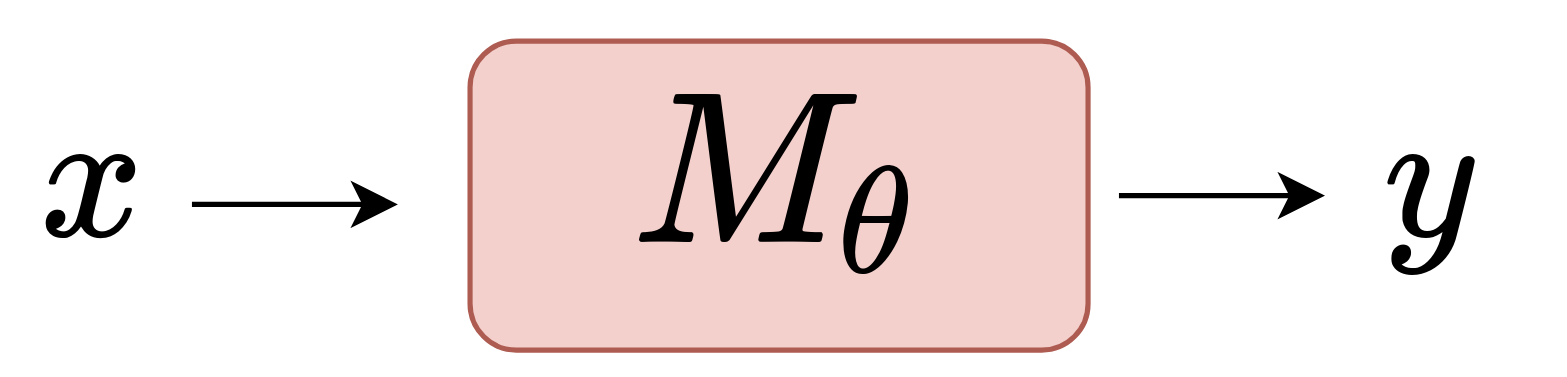
\includegraphics[width=0.85\textwidth]{fig/sup_learning.png}
\end{frame}

\begin{frame}[t]{Comparison with Supervised Learning}
  In meta learning, we have a dataset of datasets (aka, dataset distribution) $\mathcal{D} = \lbrace D_1, D_2, \cdots D_k \rbrace$, we train a model that can
  \center 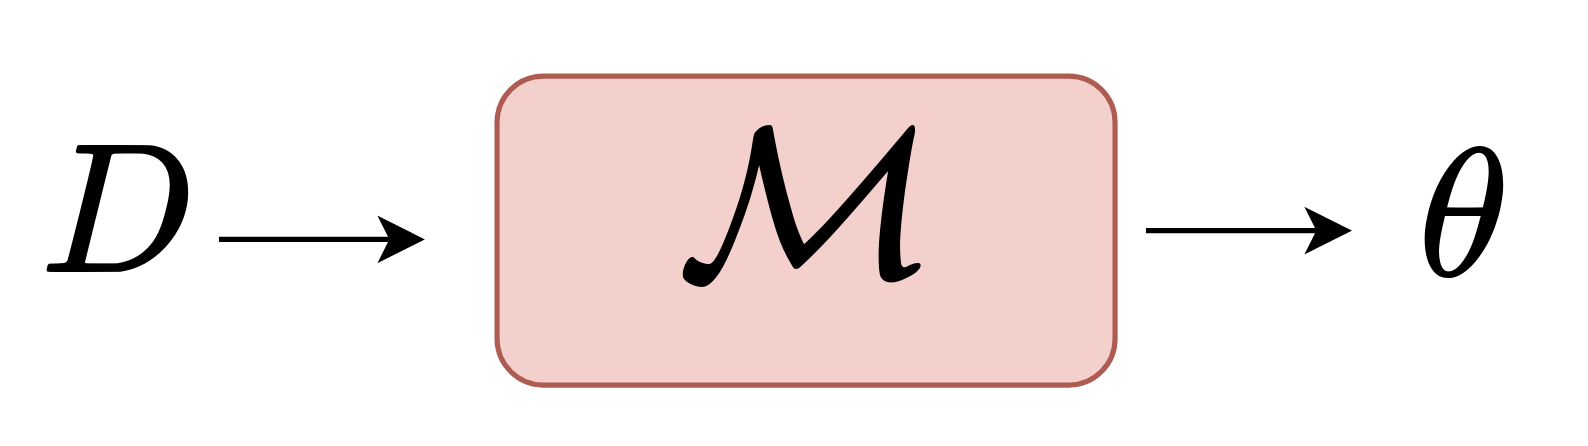
\includegraphics[width=0.85\textwidth]{fig/meta_learning.png}

  Each $D$ is not large (few-shot, low-resource)
\end{frame}

\begin{frame}[t]{What we meta-learn for?}
  \centering Meta-learn \textcolor{navy}{X} (related to $\mathcal{M}$) to improve learn \textcolor{tomato}{Y} (to get $\theta$)
  \pause
  \flushleft \textcolor{navy}{X} (what people have to decide in learning algorithm) can be
  \begin{itemize}
    \item parameter initialization
    \item optimization strategy (e.g optimizer)
    \item network architecture
    \item distance metric
    \item hyper-parameter
  \end{itemize}
\end{frame}

\begin{frame}[t]{What we meta-learn for?}
  \centering Meta-learn \textcolor{navy}{X} to improve learn \textcolor{tomato}{Y}

  \flushleft \textcolor{tomato}{Y} (application) can be
  \begin{itemize}
    \item Computer Vision
    \item Reinforcement Learning
    \item Machine Translation
    \item Dialogue Generation
    \item \textbf{Speech Recognition} (ICASSP 2020)
  \end{itemize}
  Please refer to \href{https://sunprinces.github.io/interspeech2020-meta-learning/}{HLP for meta learning}\footnote{https://sunprinces.github.io/interspeech2020-meta-learning/} for more detail
\end{frame}


\section{專題}
\begin{frame}[t]{專題規劃}
  \begin{block}{階段一: 背景知識}
    \begin{itemize}
      \item 線上課程 (metric-based, optimization-based, blackbox adaptation)
      \item 文獻閱讀 (除了上述網頁文獻,在 17 年以後的 ML 頂會文章)
    \end{itemize}
  \end{block}
\end{frame}

\begin{frame}[t]{專題規劃}
  \begin{block}{階段二: 決定題目}
    \begin{itemize}
      \item Application \& Implementation
        \begin{itemize}
          \item 找一個自己有興趣的應用,套用一個 meta learning 的方法去解決它
          \item multi modalities
        \end{itemize}
      \item Analysis
        \begin{itemize}
          \item meta-learn 出來的 model 為什麼會比較好
          \item 現行的 meta learning algorithm 有什麼問題,如何去 regularize?
          \item 提出新的 meta learning algorithm (theoretical guarantee/ efficiency)
        \end{itemize}
    \end{itemize}
  \end{block}
\end{frame}

\begin{frame}[t]{聯絡我}
  \begin{itemize}
    \item mail: sunprince12014@gmail.com
    \item 主旨: [Meta Learning 專題] 系級\_名字
    \item 內文: 你覺得該讓我知道的事(?) e.g 想做的方向,之前的相關經驗...
    \item 如果想組隊,一個人寄信即可 (在內文告知隊友還有誰)
  \end{itemize}
\end{frame}
%\begin{frame}[t]{What we meta-learn for?}
  %\centering Meta-learn \textcolor{navy}{parameter initialization} \\ to improve learn \textcolor{tomato}{End-to-End Speech Recognition}

  %\pause
  %\flushleft How to meta-learn \textcolor{navy}{parameter initialization}?
  %\begin{itemize}
    %\item Model-Agnostic Meta-Learning (MAML) (\citealt{finn2017model})
    %\item View different languages' as different tasks
  %\end{itemize}

  %\pause

  %Why \textcolor{tomato}{End-to-End Speech Recognition}?
  %\begin{itemize}
    %\item Voracious for training data
    %\item Low-resource 
  %\end{itemize}
%\end{frame}

\end{document} 
